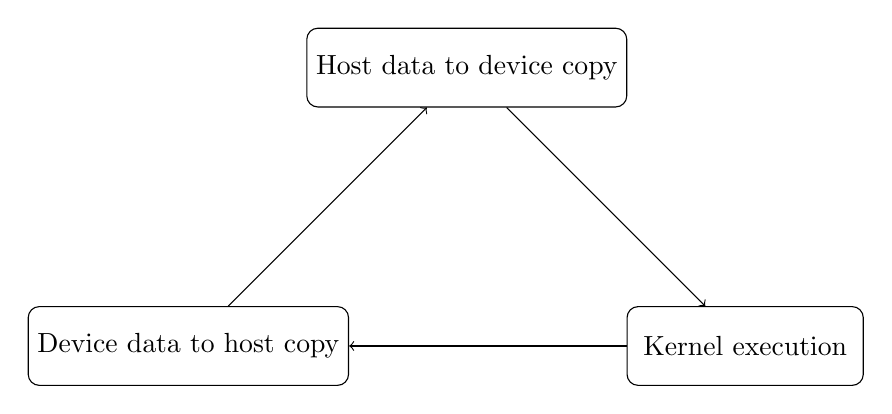
\begin{tikzpicture}[node distance=5cm]
	%defines
	\tikzstyle{hostToDevice} 	= [rectangle, rounded corners, minimum width=3cm, minimum height=1cm,text centered, draw=black]
	\tikzstyle{kernelExecution}	= [rectangle, rounded corners, minimum width=3cm, minimum height=1cm,text centered, draw=black]
	\tikzstyle{deviceToHost}	= [rectangle, rounded corners, minimum width=3cm, minimum height=1cm,text centered, draw=black]
	\tikzstyle{arrow} = [thick,->,>=stealth]
	%chart
	\node (hostToDevice) [hostToDevice] {Host data to device copy};
	\node (kernelExecution) [kernelExecution, below right of=hostToDevice] {Kernel execution};
	\node (deviceToHost) [deviceToHost, below left of=hostToDevice] {Device data to host copy};
	\draw [->] (hostToDevice) edge (kernelExecution) (kernelExecution) edge (deviceToHost) (deviceToHost) edge (hostToDevice);
\end{tikzpicture}